\section{Методика коррекции конечно-элементных моделей ЛА}

\begin{frame}{Принципиальная схема коррекции}
	\begin{center}
		\begin{tikzpicture}[scale = 1]
			\pgfmathsetmacro{\nodeDist}{0.1}
			\pgfmathsetmacro{\shiftText}{0.0}
			% Исходная модель
			\node[inner sep = 0pt] (initial) at (0, 0) {\includegraphics[width = 0.3\textwidth]{simple-model-initial}};
			\node[inner sep = 0pt, below = \shiftText of initial.south] (textInitial) {Исходная модель};
			% Знак
			\node [font = \fontsize{30}{32}, below = \nodeDist of textInitial.south, color = blue] (sumSign) {\bfseries +};
			% Коррректирующие элементы
			\node[inner sep = 0pt, below = -\nodeDist of sumSign.south] (elements) {\includegraphics[width = 0.3\textwidth]{simple-model-elements}};
			\node[inner sep = 0pt, below = \shiftText of elements.south] (textElements) {Корректирующие элементы};
			% Скорректированная модель
			\draw (sumSign.east) ++ (2.25, 0) node [right] (updated) {\includegraphics[width = 0.5\textwidth]{simple-model-updated}};
			\draw [line width = 0.75mm, -{Latex[length = 6mm]}, color = red](sumSign.east) ++ (1.25, 0) --++ (1.75, 0);
			\node[inner sep = 0pt, below = \shiftText of updated.south] (textUpdated) {Скорректированная модель};
		\end{tikzpicture}
	\end{center}
\end{frame}

\begin{frame}{Методика коррекции конечно-элементной модели}
	\begin{block}{Обобщенная проблема собственных значений}
		\begin{equation}
			(\mat{K} - \lambda \mat{M}) \mat{Y} = 0,
		\end{equation}
		где $ \mat{K} $, $ \mat{M} \in \set{R} ^ {n \times n}$~---~матрицы жесткости и масс; $ \mat{Y} $~---~формы собственных колебаний; $ \lambda $~---~собственные числа; $ N $~---~число степеней свободы.
	\end{block}
	\begin{block}{Корректирующая матрица жесткости в общем виде}
 		\begin{equation}
 			\begin{gathered}
 				\Delta \mat{K} = \Delta \internal{\mat{K}} + \Delta \external{\mat{K}}, \\
				\Delta \internal{\mat{K}}_j = \sum\limits_{p\,=\,1}^{q} \internal{c}_{j+p-1} \mat{G}_j^{(p)}, \ j = 1 \hdots e, \\
				\Delta \external{\mat{K}} = \operatorname{diag} \cbrackets{\external{c}_1, \external{c}_2, \hdots, \external{c}_N}.
			\end{gathered}
		\end{equation}
		где $ \internal{\mat{c}} $ и $ \external{\mat{c}} $~---~неизвестные внутренние и внешние корректирующие жесткости; $ \mat{G}_j^{(p)} $~---~матрица внутреннего коррректирующего элемента, составленная из длин и направляющих косинусов; $ q $~---~число корректирующих жесткостей, описывающих элемент; $ e $~---~число внутренних корректирующих элементов.
	\end{block}
\end{frame}

\begin{frame}{Внутренний корректирующий элемент в виде балки}
	\begin{block}{Матрицы корректирующего элемента}
		\begin{equation*}
		\begingroup
		\setlength\arraycolsep{2pt}
		\begin{gathered}
			\mat{G}_j^{(1)} =
			\begin{pmatrix}
				\mat{D}_1 & \mat{0} & -\mat{D}_1 & \mat{0} \\
				\mat{0} & \mat{0} & \mat{0} & \mat{0} \\
				-\mat{D}_1 & \mat{0} & \mat{D}_1 & \mat{0} \\
				\mat{0} & \mat{0} & \mat{0} & \mat{0} \\
			\end{pmatrix},
			\mat{G}_j^{(2)} =
			\begin{pmatrix}
				6 \mat{D}_2 & 3 \ell \mat{D}_4 & -6 \mat{D}_2 & 3 \ell \mat{D}_4 \\
				3 \ell \trans{\mat{D}}_4 & 2 \ell ^ 2 \mat{D}_3 & -3 \ell \trans{\mat{D}}_4 & \ell ^ 2 \mat{D}_3 \\
				-6 \trans{\mat{D}}_2 & -3 \ell \mat{D}_4 & 6 \mat{D}_2 & -3 \ell \mat{D}_4 \\
				3 \ell \trans{\mat{D}}_4 & \ell ^ 2 \trans{\mat{D}}_3 & -3 \ell \trans{\mat{D}}_4 & 2 \ell ^ 2 	\mat{D}_3
			\end{pmatrix}, \\
			\mat{G}_j^{(3)} =
			\begin{pmatrix}
				6 \mat{D}_3 & -3 \ell \trans{\mat{D}}_4 & -6 \mat{D}_3 & -3 \ell \trans{\mat{D}}_4 \\
				-3 \ell \mat{D}_4 & 2 \ell ^ 2 \mat{D}_2 & 3 \ell \mat{D}_4 & \ell ^ 2 \mat{D}_2 \\
				-6 \trans{\mat{D}}_3 & 3 \ell \trans{\mat{D}}_4 & 6 \mat{D}_3 & 3 \ell \trans{\mat{D}}_4 \\
				-3 \ell \mat{D}_4 & \ell ^ 2 \trans{\mat{D}}_2 & 3 \ell \mat{D}_4 & 2 \ell ^ 2 \mat{D}_2
			\end{pmatrix},
			\mat{G}_j^{(4)} =
			\begin{pmatrix}
				\mat{0} & \mat{0} & \mat{0} & \mat{0} \\
				\mat{0} & \mat{D}_1 & 0 & -\mat{D}_1 \\
				\mat{0} & \mat{0} & \mat{0} & \mat{0} \\
				\mat{0} & -\mat{D}_1 & 0 & \mat{D}_1 \\
			\end{pmatrix},
		\end{gathered}
		\endgroup
		\end{equation*}
	\end{block}
	\begin{block}{Матрицы из направляющих косинусов}
		\begin{equation*}
			\mat{D}_k = 
			\begin{pmatrix}
				d_{k, 1}^2 & d_{k, 1} d_{k, 2} & d_{k, 1} d_{k, 3} \\
				d_{k, 2} d_{k, 1} & d_{k, 2} ^ 2 & d_{k, 2} d_{k, 3} \\
				d_{k, 3} d_{k, 1} & d_{k, 3} d_{k, 2} & d_{k, 3} ^ 2
				\end{pmatrix},
			\mat{D}_4 = 
			\begin{pmatrix}
				d_{2, 1} d_{3, 1} & d_{2, 1} d_{3, 2} & d_{2, 1} d_{3, 3} \\
				d_{2, 2} d_{3, 1} & d_{2, 2} d_{3, 2} & d_{2, 2} d_{3, 3} \\
				d_{2, 3} d_{3, 1} & d_{2, 3} d_{3, 2} & d_{2, 3} d_{3, 3}
			\end{pmatrix},
		\end{equation*}
	\end{block}
	где $ \ell $~---~длина корректирующего балочного элемента, $ k = 1 \hdots 3 $.
\end{frame}

\begin{frame}{Расчет корректирующих жесткостей}
	\begin{block}{Задача безусловной минимизации}
		\vspace{-1em}
		\begin{gather}
			f_j(c) = \mat{Y}_j^{(0)\mathsf{T}} \Delta \mat{K}^{(i+1)} \mat{Y}_j^{(i)} + \mat{Y}_j^{(0)\mathsf{T}} \mat{K} \Delta \mat{Y}_j^{(i)} - \Delta \lambda^*_j, \\
			F(c) = \sum \limits_{j\,=\,1}^s w_j f_j^2(c) + w_c \sum \limits_{k\,=\,1}^m c_k^2 \rightarrow \min_{c},
		\end{gather}
		где $ i $~---~номер текущей итерации, $ \Delta \lambda^*_j = \lambda_j^* - \lambda_{j0} $ ($\lambda_j^*$~---~целевые собственные значения), $ w_j $~---~весовые коэффициенты, $ s $~---~число целевых частот, $ w_c $~---~параметр регуляризации.
	\end{block}	
	\begin{block}{Нормировка собственных векторов}
		\vspace{-1em}
		\begin{gather}
			\mat{Y}^{(0)\mathsf{T}} \mat{M} \mat{Y}^{(0)} = 1, \\
			\mat{Y}^{(0)\mathsf{T}} \mat{M} \mat{Y}^{(i)} = 1 \Longrightarrow \mat{Y}^{(0)T} \mat{M} \Delta \mat{Y}^{(i)} = 0,
		\end{gather}
		где $ \mat{Y}^{(0)} $, $ \mat{Y}^{(i)} $~---~исходные и текущие собственные вектора.
	\end{block}	
\end{frame}

\section{Оценка чувствительности методики коррекции}

\begin{frame}{Оценка чувствительности методики коррекции}
	\textbf{\underline{Задача}}: оценить влияние погрешностей в экспериментальном определении частот на устойчивость результата коррекции. \\ \vspace{0.5em}
	\textbf{\underline{Алгоритм оценки:}}
	\begin{enumerate}
		\item Вычисление частот и форм собственных колебаний исходной модели.
		\item Варьирование числа корректируемых тонов собственных колебаний и внесение случайных отклонений $ \Delta \mat{f} \sim \set{N} \rbrackets{\mu, \sigma ^ 2} $ в значения частот. 
		\item Решение задачи коррекции. Определение максимальной погрешности критерия модального соответствия $ \varepsilon_{\mathrm{MAC}} $ между исходными и полученными формами колебаний.
		\item Оценка первого центрального момента $ \mu_1\rbrackets{\varepsilon_{\mathrm{MAC}}} $ в зависимости от числа независимых испытаний с целью получения достоверных оценок математического ожидания и дисперсии. 
		\item Последовательность шагов 2~--~4 повторяется до тех пор, пока $ \mu_1\rbrackets{\varepsilon_{\mathrm{MAC}}} $, рассчитанный для выборки из последних наблюдений, не стабилизируется с заданной точностью.
	\end{enumerate}
\end{frame}

\begin{frame}{Оценка чувствительности методики коррекции}
	На примере свободной прямоугольной пластины показано, что:
	\begin{itemize}
		\item Методика устойчива во всем диапазоне вносимых погрешностей. 
		\item Результирующие кривые стремятся к огибающей, соответствующей предельному решению.
	\end{itemize}	
	\begin{center}
		\begin{columns}
			\begin{column}{0.5\textwidth}
				\centering
				\begin{figure}
					\begin{tikzpicture}[scale = 1]
						\hspace{-0.5em}
						\begin{semilogyaxis}[
							xlabel           = {$\Delta \mat{f} $, \% },
							ylabel           = {$ \varepsilon_{\mathrm{MAC}} $, \%},
							ylabel shift     = -5 pt,
							grid             = major,
							legend columns   = 3,
							legend style     = {
								at           = {(0.65, 0.03)},
								anchor       = south,
								fill         = white,
								fill opacity = 0.6,
								draw opacity = 1,
								text opacity = 1,
							},
							ylabel near ticks,  
							xtick            = {0, 1, 2, 3, 4, 5},
							ytick            = {1e-6, 1e-4, 1e-2, 1e0},
							mark size        = 1.1pt,
							width            = 6.1cm
						]
							\pgfplotstableread{images/partModelUpdating/perturbation-plate-errors.txt}\contentFile
							\addplot[color = blue, mark = *] table [x index = 0, y index = 1] {\contentFile};
							\addplot[color = red, mark = triangle*] table [x index = 0, y index = 2] {\contentFile};
							\addplot[color = olive, mark = diamond*] table [x index = 0, y index = 3] {\contentFile};
							\addplot[color = purple, mark = halfcircle*] table [x index = 0, y index = 4] {\contentFile};
							\addplot[color = teal, mark = x] table [x index = 0, y index = 5] {\contentFile};
							\legend{$ 1 $, $ 3 $, $ 5 $, $ 7 $, $ 9 $}
						\end{semilogyaxis}
					\end{tikzpicture}
					Погрешность определения форм колебаний свободной пластины
				\end{figure}
			\end{column}
			\hfill
			\begin{column}{0.5\textwidth}
				\centering
				\vspace{-1.8em}
				\begin{figure}
					\begin{tikzpicture}[scale = 1]
						\hspace{-1em}
						\begin{axis}[
							xlabel           = {$\Delta \mat{f} $, \% },
							ylabel           = {$ N_\Sigma $},
							ylabel shift     = -10 pt,
							legend columns   = 1,
							legend style     = {
								at           = {(0.05, 0.65)},
								anchor       = west,
								fill         = white,
								fill opacity = 0.6,
								draw opacity = 1,
								text opacity = 1,
							},
							ylabel near ticks,
							try min ticks = 6,
							bar width  = 2pt,
							width      = 6.1cm,
							ybar stacked,
							scaled y ticks = base 10:-3,
							tick scale binop = \times,
				          	xmin = 0.15, xmax = 5.05, ymin = 0
						]
							\pgfplotstableread{images/partModelUpdating/perturbation-plate-samplesize.txt}\contentFile
							\addplot table [x index = 0, y index = 1] {\contentFile};
							\addplot table [x index = 0, y index = 2] {\contentFile};
							\addplot table [x index = 0, y index = 3] {\contentFile};
							\addplot table [x index = 0, y index = 4] {\contentFile};
							\addplot table [x index = 0, y index = 5] {\contentFile};
							\legend{$ 1 $, $ 3 $, $ 5 $, $ 7 $, $ 9 $}
						\end{axis}
					\end{tikzpicture}
					Число независимых испытаний свободной пластины
				\end{figure}
			\end{column}
		\end{columns}
	\end{center}
\end{frame}

\section{Способ освобождения КЭ-моделей от закреплений}

\begin{frame}{Способ освобождения КЭ-модели от закреплений}
	\begin{equation} 
		\begin{pmatrix}
			\mat{K} & -(\sum \mat{k})^\intercal \\
			 -\sum \mat{k} & \mat{0} 
		\end{pmatrix} 
		\begin{Bmatrix}
			\tilde{X} \\ 
			\xi
		\end{Bmatrix}			
		+ 
		\begin{pmatrix}
			\mat{M} & \mat{0} \\
			\mat{0} & \mu - \sum \sum \mat{m}
		\end{pmatrix}
			\begin{Bmatrix}
			\ddot{\tilde{\mat{X}}} \\ 
			\ddot{\mat{\xi}}
		\end{Bmatrix}	
		= 0,
	\end{equation}
	где $ \sum k = F_s(\mat{K}) \in R ^ {6 \times n}$, $ \sum \sum m = F_m(F_s(\mat{M})) \in R ^ {6 \times 6} $~---~дополнительные матричные элементы.
	\begin{center}
		\begin{tikzpicture}[scale = 1]
			\pgfmathsetmacro{\nodeDist}{0.2}
			\pgfmathsetmacro{\shiftText}{0.01}
			\tikzstyle{arrow} = [draw, line width = 0.75mm, -{Latex[length = 6mm]}] 
			% Су-34
			\node[inner sep = 0pt] (spring) at (0, 0) {\includegraphics[width = 0.35\textwidth]{spring-su-34}};
			\node[inner sep = 0pt, below = \shiftText of spring.south] (textSpring) {Испытания на упругой подвеске};
			\draw (spring.east) ++ (1.5, 0) node [right] (freeSu34) {\includegraphics[width = 0.3\textwidth]{free-su-34}};
			% Як-152
			\node[inner sep = 0pt, below = \nodeDist of textSpring.south] (gear) {\includegraphics[width = 0.35\textwidth]{gear-yak-152}};
			\node[inner sep = 0pt, below = \shiftText of gear.south] (textGear) {Испытания на шасси};
			\draw (gear.east) ++ (1.5, 0) node [right] (freeYak152) {\includegraphics[width = 0.3\textwidth]{free-yak-152}};
			\node[inner sep = 0pt, below = \shiftText of freeYak152.south] (textFree) {После освобождения};
			% Стрелки
			\draw [arrow, color = red](spring.east) ++ (0.2, 0) --++ (1.3, 0);
			\draw [arrow, color = blue](gear.east) ++ (0.2, 0) --++ (1.3, 0);
		\end{tikzpicture}
	\end{center}
\end{frame}

\section{Положения, выносимые на защиту}

\begin{frame}{Положения, выносимые на защиту}
	\begin{enumerate}
		\item Методика коррекции конечно-элементных моделей ЛА, заключающаяся в добавлении корректирующих конечных элементов, параметры которых определяются по результатам модальных испытаний.
		\item Способ определения частот и форм собственных колебаний свободной конструкции по результатам испытаний этой конструкции с наложенными связями.
	\end{enumerate}
\end{frame}

\section{Методика синтеза расчетной модели конструкции из ее составных частей}

\begin{frame}{Методика синтеза глобальных расчетных моделей конструкций}
	\begin{center}
		\begin{columns}
			\begin{column}{0.5\textwidth}
				\centering
				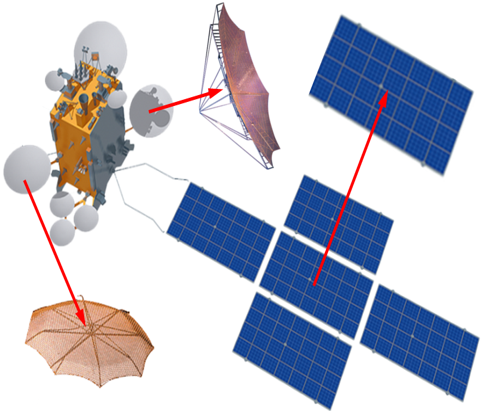
\includegraphics[width = 1\textwidth]{images/synopsis/decomposition}
			\end{column}
			\begin{column}{0.5\textwidth}
				\centering
				% Определение стиля
				\tikzstyle{blockWide}=[rectangle, draw = black, fill = blue!20, rounded corners, text width = 20em, text centered, minimum height = 1.5em, drop shadow] % Блок
				\tikzstyle{blockWideC}=[blockWide, fill = red!20]
				\tikzstyle{arrow} = [draw, thick, color=black!90, -latex'] % Стрелка
				\scriptsize % Размер шрифта
				% Задание перменных
				\def\nodeDist{0.3cm} % Дистанция между узлами
				% Отрисовка блок-схемы
				\begin{tikzpicture}[scale = 1, transform shape]
					% Задание узлов		
					\node (modalTests) [blockWide] {Модальные испытания составных частей конструкции};
					\node (modelUpdating) [blockWide, below = \nodeDist of modalTests] {Коррекция расчетных моделей составных частей конструкции по результатам испытаний};
					\node (checkInfluence) [blockWide, below = \nodeDist of modelUpdating] {Освобождение закрепленных расчетных моделей составных частей конструкции};
					\node (buildRealModel) [blockWide, below = \nodeDist of checkInfluence] {Синтез расчетной модели полной конструкции из её составных частей};
					\node (buildMathModel) [blockWide, below = \nodeDist of buildRealModel] {Определение динамических характеристик полной расчетной модели};
					% Соединение узлов
					\draw [arrow] (modalTests.south) -- (modelUpdating.north);
					\draw [arrow] (modelUpdating.south) -- (checkInfluence.north);
					\draw [arrow] (checkInfluence.south) -- (buildRealModel.north);
					\draw [arrow] (buildRealModel.south) -- (buildMathModel.north);
				\end{tikzpicture}
			\end{column}
		\end{columns}
		\vspace{0.2em}
		Схема методики синтеза глобальных расчетных моделей
	\end{center}
	\vspace{-0.6em}
	\begin{block}{Достоинства методики}
		\begin{itemize}
			\setlength{\itemsep}{0pt}
			\item Составные части обладают более высокими частотами собственных колебаний.
			\item Не требуется больших помещений для проведения испытаний.
			\item Меньшее влияние воздушной среды на определяемые динамические характеристики.
		\end{itemize} 
	\end{block}
\end{frame}

\begin{frame}{Построение матриц демпфирования составных частей}
	\begin{center}
		\begin{columns}
			\begin{column}{0.54\textwidth }
				\centering
				\vspace{-0.75em}
				\includegraphics[width = 1\textwidth]{ms-21}
				Модальные испытания МС-21
			\end{column}
			\begin{column}{0.45\textwidth}
				\centering
				\begin{tikzpicture}[scale = 1]
					\small
					\pgfmathsetmacro{\vertStep}{0.6}
					\begin{axis}[
						xlabel            = {$ \overline{f} $},
						ylabel            = {$ \lambda $}, 
						ylabel shift      = -5 pt,
						width             = 5.7cm,
						grid              = both,
						mark size         = 1pt,
						ylabel near ticks,
						xlabel near ticks,
						xmin = 0.985, xmax = 1.025
					]
						\pgfplotstableread{images/presentation/monophase-parameter.txt}\contentFile
						\addplot table [x index = 0, y index = 1] {\contentFile};
						\addplot table [x index = 0, y index = 2] {\contentFile};
						\node[text width = 25mm] at (axis cs: 1.012, -1.55) {Вертикальный изгиб фюзеляжа};
						\draw[very thick, dashed, color = teal] (axis cs:1, -\vertStep) -- (axis cs:1, \vertStep);
						\node[color = teal] at (axis cs: 0.996, 0.5) {$ \overline{f}_\text{рез} $};
					\end{axis}
				\end{tikzpicture}
			\end{column}
		\end{columns}
	\end{center}
	\vspace{-1em}
	\begin{block}{Нулевое приближение по гипотезе Сорокина}
		\begin{equation}
			\begin{gathered}
			\mat{H} = \alpha \tilde{\mat{K}} + \beta \mat{M}, \\
			G(\alpha, \beta) = \sum\limits_{i\,=\,1}^p w_i \left( 1 - \frac{\alpha \tilde{\kappa}_i + \beta \mu_i}{h_i} \right)^2 \rightarrow \min_{\alpha, \beta}.
			\end{gathered}
		\end{equation}
	\end{block}
	\vspace{-0.5em}
	\begin{block}{Введение корректирующих элементов}
		\begin{equation}
			\tilde{\mat{H}} = \mat{H} + \Delta \internal{\mat{H}} + \Delta \external{\mat{H}}.
		\end{equation}
	\end{block}
\end{frame}

\begin{frame}{Тестирование методики синтеза на примере модели КА}
	\begin{center}
		\begin{tikzpicture}
			\pgfmathsetmacro{\horizDist}{5}
			\pgfmathsetmacro{\vertDist}{0.75}
			\pgfmathsetmacro{\shiftText}{0.01}
			\tikzstyle{arrow} = [draw, line width = 0.5mm, -{Latex[length = 3mm]}, color = blue] 
			% Полная модель
			\node[inner sep = 0pt] (mesh) at (0, 0) {\includegraphics[width = 0.7\textwidth]{images/presentation/spacecraft-test-mesh}};
			\node[inner sep = 0pt, below = \shiftText of mesh.south] (textMesh) {Глобальная модель};
			% Орбитальный модуль
			\draw (mesh.south) ++ (-\horizDist/2, -\vertDist) node [below] (orbital) {\includegraphics[width = 0.35\textwidth]{test-spacecraft-orbital-distribution}};
			\node[inner sep = 0pt, below = \shiftText of orbital.south] (textOrbital) {а) Орбитальный модуль};
			% Панели солнечных батарей
			\draw (mesh.south) ++ (\horizDist/2, -\vertDist) node [below] (panel) {\includegraphics[height = 0.33\textwidth]{test-spacecraft-panel-distribution}};
			\node[inner sep = 0pt, below = \shiftText of panel.south] (textPanel) {б) Панели солнечных батарей};
			% Стрелки
			\draw [arrow] (textMesh.west) ++ (-0.3, 0) -- (orbital.north);
			\draw [arrow] (textMesh.east) ++ (0.3, 0) -- (panel.north);
		\end{tikzpicture}
		
		Изменения узловых жесткостей при коррекции моделей составных частей
	\end{center}	
\end{frame}

\begin{frame}{Результаты синтеза глобальной модели КА}
	\begin{center}
		\begin{columns}
			\begin{column}{0.47\textwidth}
				\centering
				\small
				\begin{tikzpicture}[scale = 1]
					\hspace{-0.5em}
					\begin{semilogyaxis}[
						xlabel            = {Номер итерации коррекции},
						ylabel            = {$ \lVert \mat{\alpha} \rVert_{\max} $}, 
						ylabel shift      = -5 pt,
						width             = 6.25cm,
						grid              = both,
						legend cell align = left,
						legend style      = {
							at            = {(0.02, 0.14)},
							anchor        = west,
							fill          = white,
							fill opacity  = 0.6,
							draw opacity  = 1,
							text opacity  = 1,
						},
						ylabel near ticks,
						xmin = 0, xmax = 8
					]
						\addplot table {images/partModelUpdating/test-spacecraft-panels-convergence.txt};
						\addplot table {images/partModelUpdating/test-spacecraft-orbital-convergence.txt};
						\legend{Панели, Орбитальный модуль}
					\end{semilogyaxis}
				\end{tikzpicture}
				Оценка сходимости коррекции по частотному критерию
			\end{column}
			\hfill
			\begin{column}{0.52\textwidth}		
				\centering
				\begin{tblr}{
					colspec = {|X[c, -1]|X[c]|X[c]|X[c]|X[c]|},
					hlines,
					colsep = 1pt,
					rows = {font = \footnotesize}
				}
					\SetCell[r = 3]{c} Тон & \SetCell[c = 4]{c} Погрешность в частотах, \% &&& \\
					& \SetCell[r = 2]{c} Исходная & \SetCell[c = 3]{c} После коррекции && \\
					& & Панелей & Модуля & {Панелей \\ и модуля} \\ \hline
					7 & -4.689 & -2.120 & -2.756 & -0.021 \\
					8 & -4.678 & -2.078 & -2.782 & -0.018 \\
					9 & -5.121 & -4.447 & -0.674 & 0.100  \\
					10 & -5.040 & -4.760 & -0.354 & -0.028 \\
					11 & -5.040 & -4.760 & -0.357 & -0.032 \\
					12 & -5.121 & -4.443 & -0.687 & 0.091 \\
					13 & -4.102 & -0.966 & -3.161 & 0.011 \\
					14 & -4.112 & -0.999 & -3.135 & 0.016 \\
					15 & -3.303 & -0.234 & -3.066 & -0.006 \\
					16 & -3.303 & -0.234 & -3.066 & -0.005 \\
				\end{tblr}
			\end{column}
		\end{columns}
	\end{center}
\end{frame}

\section{Положения, выносимые на защиту (продолжение)}

\begin{frame}{Положения, выносимые на защиту}
	\begin{enumerate}
		\setcounter{enumi}{2} 
		\item Обоснована методика формирования глобальной матрицы демпфирования конструкций по результатам испытаний их составных частей.
		\item Развита методика испытаний составных частей ЛА для достоверного построения их матриц жесткости.
	\end{enumerate}
\end{frame}

\section{Программы для обработки и представления результатов модальных испытаний}

\begin{frame}{Программы для обработки и представления результатов модальных испытаний}
	\begin{center}
		\begin{tikzpicture}
			\node[inner sep = 0pt] (gencalc) at (0, 0) {\includegraphics[width = 0.6\textwidth]{gencalc-interface}};
			\node[inner sep = 0pt] (analyzer) at (3, -2) {\includegraphics[width = 0.6\textwidth]{analyzer-interface}};
		\end{tikzpicture}
	\end{center}
\end{frame}

\section{Программа для диагностирования дефектов конструкций по результатам испытаний}

\begin{frame}{Программа для диагностирования дефектов конструкций по результатам испытаний}
	Возможное месторасположение дефекта соответствует максимуму параметра искажений портретов колебаний. Типы обнаруживаемых дефектов: зазоры, люфты и трещины. 
	\begin{center}
		\begin{figure}
			\begin{subfigure}[t]{0.53\textwidth}
				\includegraphics[width = 1\textwidth]{express-amu-7}
			\end{subfigure}
			\begin{subfigure}[t]{0.45\textwidth}
				\includegraphics[width = 1\textwidth]{distortion-spacecraft}
			\end{subfigure}
		\end{figure}
		Обнаружение зазоров в узлах установки солнечных батарей
	\end{center}
\end{frame}

\section{Операционный модальный анализ по результатам летных испытаний}

\begin{frame}{Операционный модальный анализ по результатам летных испытаний}

	\begin{center}
		\begin{columns}
			\begin{column}{0.55\textwidth}
				\centering
				\textbf{Методика определения критической скорости флаттера}:
				\begin{itemize}
					\setlength{\itemsep}{0pt}
					\raggedright
					\item выход летательного аппарата на исследуемый скоростной режим;
					\item задание генератором сигналов в систему управления; 
					\item передача системой управления воздействий отклоняемым поверхностям;
					\item регистрация колебаний тензодатчиками и акселерометрами до полного завершения переходных процессов;
					\item обобщение и обработка результатов измерений на различных скоростях полета.
				\end{itemize}
			\end{column}		
			\begin{column}{0.43\textwidth}
				\centering
				\begin{tikzpicture}[scale = 1]
					\hspace{-1em}
					\small
					\begin{axis}[
						xlabel            = {$ v $, км/ч},
						ylabel            = {$ \delta $},
						ylabel shift      = -2 pt,
						y dir             = reverse,
						grid              = major,
						legend columns    = 1,
						legend cell align = {left},
						legend style      = {
							at            = {(0.025, 0.68)},
							anchor        = west,
							fill          = white,
							fill opacity  = 0.6,
							draw opacity  = 1,
							text opacity  = 1,
						},
						ylabel near ticks,
						ymin = 0,
						x tick label style = {
							/pgf/number format/.cd,
							set thousands separator = {},
							fixed
						},
						y tick label style = {
							/pgf/number format/.cd,
							fixed
						},
						ylabel near ticks,  
						try min ticks    = 6,
						mark size        = 1.25pt,
						width            = 5.5cm,
						height           = 5.75cm,
					]
						\pgfplotstableread{images/synopsis/flight-decrements-2.txt}\contentFile
						\addplot[color = blue, thick, mark = *, smooth, tension = 0.2] table [x index = 0, y index = 1] {\contentFile};
						\addplot[color = gray, thick, mark = triangle*, smooth, tension = 0.2] table [x index = 0, y index = 2] {\contentFile};
						\addplot[color = teal, thick, mark = diamond*, smooth, tension = 0.2] table [x index = 0, y index = 3] {\contentFile};
						\addplot[color = red, thick,  mark = halfcircle*, smooth, tension = 0.2] table [x index = 0, y index = 4] {\contentFile};
						\addplot[color = orange, thick, densely dashed, mark = o, mark options = {solid}, smooth, tension = 0.2] table [x index = 0, y index = 5] {\contentFile};
						\addplot[color = violet, thick, densely dashed, mark = o, mark options = {solid}, smooth, tension = 0.2] table [x index = 0, y index = 6] {\contentFile};
						\legend{\name{SSI-DD}, \name{ERA}, \name{ADA}, \name{N4SID}, {\name{ЛИИ}, оценка сверху}, {\name{ЛИИ}, оценка снизу}}
					\end{axis}
				\end{tikzpicture}
				Скоростные зависимости логарифмического декремента Су-30
			\end{column}
		\end{columns}
	\end{center}
\end{frame}

\section{Определение динамических характеристик рефлектора по результатам акустических испытаний}

\begin{frame}{Определение модальных характеристик рефлектора по результатам акустических испытаний}
	\textbf{\underline{Принимаемые гипотезы}}:
	\begin{itemize}
		\item динамическая система является стационарной;
		\item исследуемый объект является наблюдаемым: расположение датчиков на конструкции позволяет однозначно идентифицировать формы колебаний, частоты которых лежат в интересующем диапазоне.
	\end{itemize}
	\begin{center}
		\begin{figure}
			\centering
			\small
			\begin{subfigure}[t]{0.49\textwidth}
				\includegraphics[width = 1\textwidth]{reflector-experiment}
				а) Рефлектор в акустической камере
			\end{subfigure}
			\hfill
			\begin{subfigure}[t]{0.49\textwidth}
				\includegraphics[width = 1\textwidth]{reflector-sensors} 
				б) Расположение датчиков на поверхности рефлектора
			\end{subfigure}
		\end{figure}
		\vspace{0.5em}
		Проведение акустических испытаний
	\end{center}
\end{frame}

\begin{frame}{Результаты определения динамических характеристик рефлектора методами операционного модального анализа}
	\centering
	\vspace{0.5em}
	\begin{tblr}{
		colspec = {|c|c|c|c||c|c|c|},
		hlines,
		rows = {font = \footnotesize}
	}
		\SetCell[r = 2]{c} Тон & \SetCell[c = 3]{c} Частота $ f $, Гц && & \SetCell[c = 3]{c} Логарифмический декремент $ \delta $ && \\
		& SSI-COV & ERA & SSI-DD & SSI-COV & ERA & SSI-DD \\ \hline
		1 & 66.052 & 65.962 & 66.403 & 0.054 & 0.042 & 0.045 \\
		2 & 91.287 & 90.910 & 91.843 & 0.030 & 0.052 & 0.042 \\
		3 & 102.540 & --- & --- & 0.056 & --- & --- \\
		4 & 114.770 & --- & --- & 0.063 & --- & --- \\
		5 & 122.370 & --- & --- & 0.094 & --- & --- \\
	\end{tblr}
	\begin{columns}
		\footnotesize
		\begin{column}{0.25\textwidth}
			\centering
			\includegraphics[width = 1\textwidth]{reflector-ssi-cov-mode-1}
			$ f = 91.29 $ Гц, $ \delta = 0.03 $ 
		\end{column}
		\begin{column}{0.25\textwidth}	
			\centering
			\includegraphics[width = 1\textwidth]{reflector-ssi-cov-mode-2} 
			$ f = 127.85 $ Гц, $ \delta = 0.05 $
		\end{column}
		\begin{column}{0.25\textwidth}	
			\centering
			\includegraphics[width = 1\textwidth]{reflector-ssi-cov-mode-4} 
			$ f = 325.36 $ Гц, $ \delta = 0.03 $
		\end{column}
	\end{columns}
	\vspace{0.5em}
	Идентифицированные тона колебаний
\end{frame}

\section{Решение практических задач коррекции расчетных моделей}

\section{Коррекция расчетной модели динамически-подобной модели самолета Ту-204}

\begin{frame}{Коррекция расчетной модели динамически-подобной модели самолета Ту-204}
	Геометрические и физические характеристики модели:
	\begin{columns}
		\begin{column}{0.45\textwidth}
			\begin{itemize}
				\item Размах крыла --- $ 3172 $ мм.
				\item Длина фюзеляжа --- $ 3462 $ мм.
			\end{itemize}
		\end{column}
		\begin{column}{0.55\textwidth}
			\begin{itemize}
				\item Масштаб моделирования --- $ 1 \div 10 $.
				\item Масса модели --- $ 50.5 $ кг.
			\end{itemize}
		\end{column}
	\end{columns}
	\begin{center}
		\begin{figure}
			\small
			\begin{subfigure}[t]{0.49\textwidth}
				\centering
		     	\includegraphics[width = 1\textwidth]{tu-204-experiment} 
		     	а) Упругое вывешивание модели
		    \end{subfigure}
	    	\hfill
		    \begin{subfigure}[t]{0.49\textwidth}
				\centering
				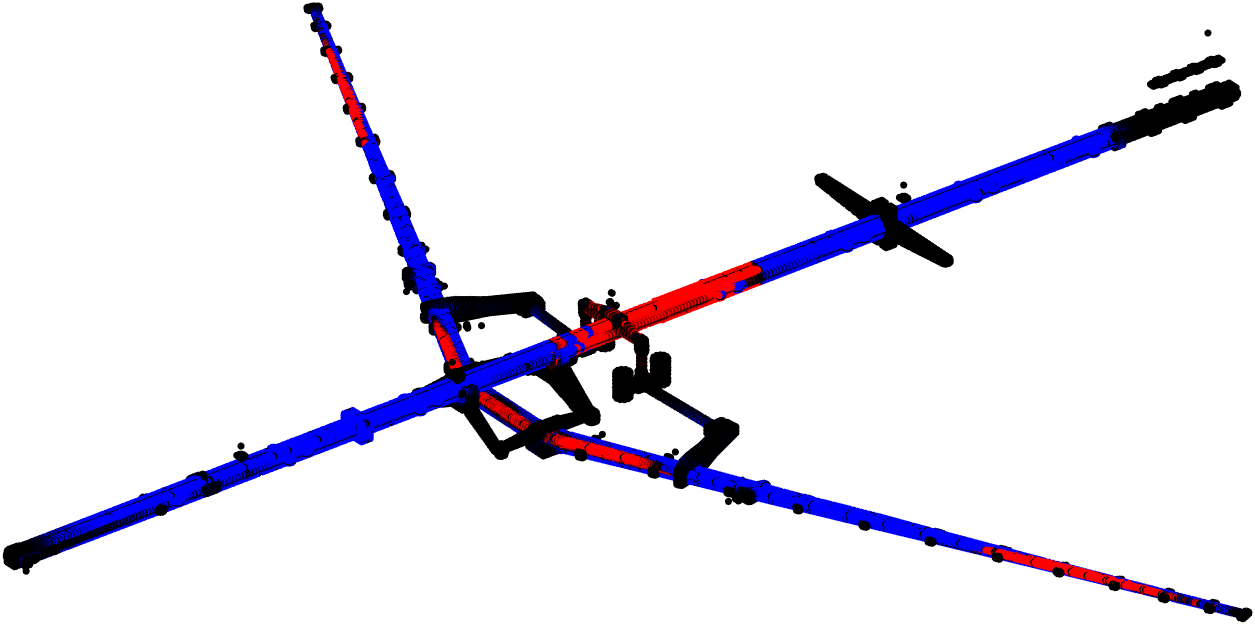
\includegraphics[width = 1\textwidth]{tu-204-coeffs-6}
				б) Изменение узловых жесткостей
		    \end{subfigure}
		\end{figure}
		\vspace{1em}
		Динамически-подобная модель самолета Ту-204
	\end{center}
\end{frame}

\begin{frame}{Результаты применения методики коррекции} 
	\resizebox{\textwidth}{!}{%
	\begin{tblr}
	{
		colspec = {|c|c|c|c|c|c|c|c|c|c|}, 
		hlines
	}
   		\SetCell[r = 3]{c} Тон & \SetCell[c = 2]{c} Частоты, Гц && \SetCell[c = 7]{c} Погрешность до и после коррекции, \%  \\
	   	& \SetCell[r = 2]{c} Эксперимент & \SetCell[r = 2]{c} {Исходная \\ модель} & \SetCell[r = 2]{c} До & \SetCell[c = 6]{c} После \\ 
   		& & & & 1 & 2 & 3 & 4 & 5 & 6 \\ \hline
		СИКр1\footnotemark[1] & 3.44 & 3.49 & 1.5 & 0.0 & 0.0 & 0.0 & 0.0 & 0.0 & 0.0 \\
		АСИКр1\footnotemark[2] & 4.87 & 4.96 & 1.7 & -0.6 & 0.0 & 0.0 & 0.0 & 0.0 & 0.0 \\
		ГИФ1\footnotemark[3] & 5.44 & 5.73 & 5.3 & 4.7 & 4.7 & 0.0 & 0.0 & 0.0 & 0.0 \\ 
		ВИФ1\footnotemark[4] & 5.73 & 5.97 & 4.2 & 3.5 & 3.3 & 2.6 & 0.0 & 0.0 & 0.0 \\
		СИКр2\footnotemark[5] & 9.30 & 9.13 & -1.8 & -4.4 & -3.2 & -3.9 & -4.4 & 0.0 & 0.0 \\
		ВИФ2\footnotemark[6] & 14.18 & 14.77 & 4.2 & 3.7 & 3.8 & 3.4 & 2.0 & 3.3 & 0.0 \\
	\end{tblr} }
	\footnotetext[1]{Cимметричный изгиб крыла I тона}
	\footnotetext[2]{Антисимметричный изгиб крыла I тона}
	\footnotetext[3]{Горизонтальный изгиб фюзеляжа I тона}
	\footnotetext[4]{Вертикальный изгиб фюзеляжа I тона}
	\footnotetext[5]{Симметричный изгиб крыла II тона}
	\footnotetext[6]{Вертикальный изгиб фюзеляжа II тона}
\end{frame}

\section{Синтез имитационной модели каркаса зонтичной антенны космического аппарата}

\begin{frame}{Синтез имитационной модели каркаса зонтичной антенны космического аппарата}
	\begin{center}
		\begin{tikzpicture}
			\small
			\pgfmathsetmacro{\vertDist}{4}
			\pgfmathsetmacro{\shiftText}{0.05}
			\tikzstyle{arrow} = [draw, line width = 0.5mm, -{Latex[length = 2.5mm]}, color = blue] 
			% Полная модель
			\node (boundary) at (0, 0) {};
			\draw (boundary.east) ++ (3.25, 0) node (assembly) {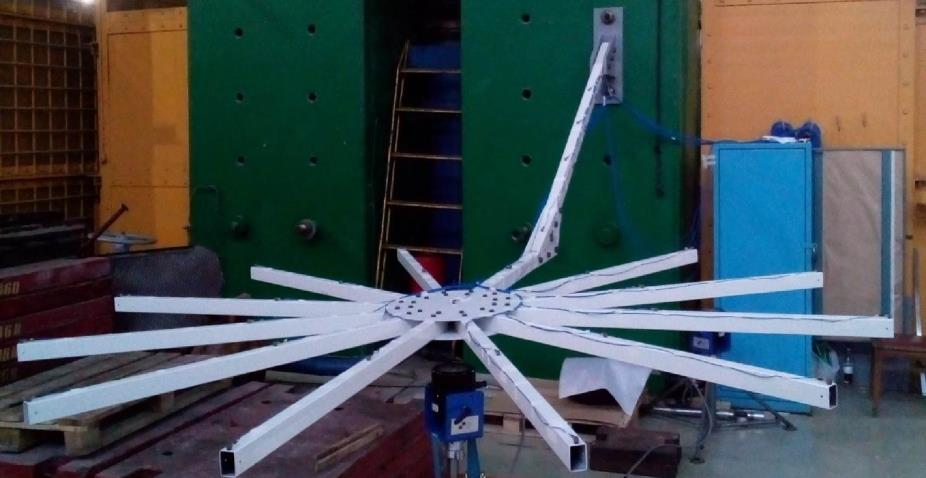
\includegraphics[width = 0.5\textwidth]{simsat-assembly}};
			\node[inner sep = 0pt, below = \shiftText of assembly.south] (textAssembly) {Конструкция в сборе};
			% Сведения
			\draw (assembly.east) ++ (5.75, 0) node (info){
				\vbox				
				{\begin{itemize}
					\item Длина штанги --- $ 2250 $ мм.
					\item Масса штанги --- 22 кг.
					\item Диаметр рефлектора --- $ 3000 $ мм.
					\item Масса рефлектора --- $ 73 $ кг.
				\end{itemize}}
			};
			% Зонтичный каркас
			\node (antenna) at (3, -\vertDist)  {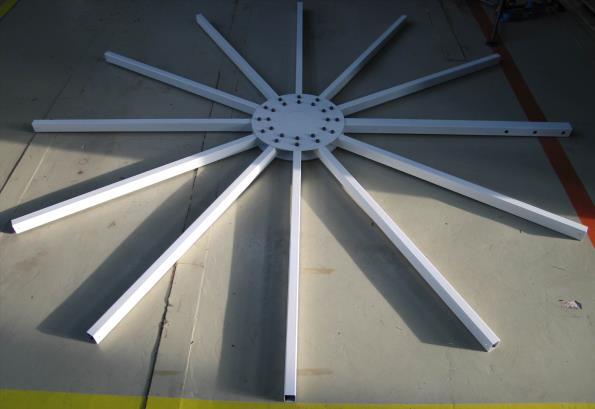
\includegraphics[width = 0.35\textwidth]{simsat-antenna}};
			\node[inner sep = 0pt, below = \shiftText of antenna.south] (textAntenna) {а) Рефлектор};
			% Штанга
			\node (handle) at (8, -\vertDist) {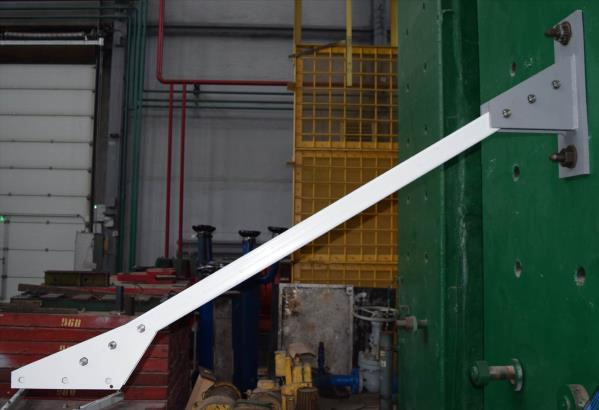
\includegraphics[width = 0.35\textwidth]{simsat-handle}};
			\node[inner sep = 0pt, below = \shiftText of handle.south] (textHandle) {б) Штанга};
			% Стрелки
			\draw [arrow] (antenna.north) ++ (0, 0.45) -- (antenna.north);
			\draw [arrow] (textAssembly.east) ++ (0.2, 0) -- (handle.north);
		\end{tikzpicture}
		
		Имитационная модель каркаса зонтичной антенны
	\end{center}
\end{frame}

\begin{frame}{Результаты применения методики синтеза} 
	\small
	\begin{center}
		\begin{columns}
			\begin{column}{0.6\textwidth}
				\centering
				\includegraphics[width = 1\textwidth]{scheme-fixture}
			\end{column}
			\begin{column}{0.4\textwidth}
				\centering
				\includegraphics[width = 0.7\textwidth]{scheme-springs}
			\end{column}
		\end{columns}
		Расчетные схемы для оценки податливости закреплений в эксперименте \\
		\vspace{0.5em}
		\begin{tblr}
		{
			colspec = {|c|c|c|c|}, 
			hlines,
			colsep = 2pt,
			rows = {font = \footnotesize}
		}
			\SetCell[r = 2]{c} Тон & \SetCell[c = 3]{c} {Погрешность до и после коррекции, \%} \\
			& Исходная & {Коррекция \\ (настоящая методика)} & {Коррекция \\ (Маринин, 2020)} \\ \hline
			1 & 1.84 & 0.70 & 0.66 \\ 
		    2 & 3.88 & 0.40 & 2.76 \\ 
		    3 & 3.19 & 1.24 & 2.97 \\ 
	    	4 & 2.13 & 1.18 & 1.78 \\ 
		    5 & 2.25 & 1.95 & 1.95 \\ 
		\end{tblr}
	\end{center}	
\end{frame}

\section{Коррекция расчетной модели отъемной части крыла изделия С-70}

\begin{frame}{Коррекция расчетной модели отъемной части крыла изделия С-70}
	\begin{center}
		\begin{figure}
			\small
			\begin{subfigure}[t]{0.35\textwidth}
				\centering
		     	\includegraphics[width = 0.7\textwidth]{images/presentation/wing-experiment} \\
		     	Консоль крыла на подвеске
		    \end{subfigure}
		    \begin{subfigure}[t]{0.45\textwidth}
				\centering
				\includegraphics[width = 1\textwidth]{wing-coeffs-5} \\
				Изменение узловых жесткостей
		    \end{subfigure}
		\end{figure}
		\vspace{0.5em}
		\begin{tblr}{
			colspec = {|c|c|c|c|c|c|c|c|c|}, 
			width = \textwidth, 
			hlines,
			rows = {font = \footnotesize}
		}
			\SetCell[r = 3]{c} Тон & \SetCell[c = 2]{c} Приведенная частота && \SetCell[c = 6]{c} Погрешность до и после коррекции, \% \\
			& \SetCell[r = 2]{c} Эксперимент & \SetCell[r = 2]{c} {Исходная \\ модель} & \SetCell[r = 2]{c} До & \SetCell[c = 5]{c}После \\
			& & & & 1 & 2 & 3 & 4 & 5 \\ \hline
			1 & 1.00 & 1.51 & 50.7 & 0.0 & 0.0 & 0.0 & 0.0 & 0.0 \\ 
			2 & 2.28 & 3.18 & 39.5 & -7.4 & 0.0 & 0.0 & 0.0 & 0.0 \\ 
			3 & 3.37 & 4.13 & 22.6 & -18.6 & -13.8 & 0.0 & 0.0 & 0.0 \\ 
			4 & 3.95 & 4.82 & 21.8 & -19.1 & -17.8 & -8.2 & 0.0 & 0.0 \\ 
			5 & 4.87 & 6.15 & 26.2 & -16.2 & -21.8 & -2.6 & -4.4 & 0.0 \\ 
		\end{tblr}
	\end{center}
\end{frame}

\begin{frame}{Сопоставление форм колебаний до и после коррекции}
	\begin{block}{Критерий модального соответствия (MAC-критерий)}
		\begin{equation}
			\mathrm{MAC}_{i, j} = \frac{(\mat{u}_i ^ \intercal \cdot \mat{v}_j) ^ 2}{(\mat{u}_i ^ \intercal \cdot \mat{u}_i) (\mat{v}_j ^ \intercal \cdot \mat{v}_j)}, 
		\end{equation}
		где $ \mat{u}_i $ и $ \mat{v}_j $~---~формы колебаний до и после коррекции; $ i, j = 1 \hdots n $.
	\end{block}
	\vspace{-0.5em}
	\begin{columns}
		\begin{column}{0.49\textwidth}
			\centering
			\begin{figure}
				\includegraphics[width=1\textwidth]{wing-MAC}
			\end{figure}
		\end{column}
		\begin{column}{0.4\textwidth}
			\centering
			\begin{figure}
				\includegraphics[width=1\textwidth]{wing-initial-mode-1} \\ \vspace{0.2em}
				\includegraphics[width=1\textwidth]{wing-initial-mode-2} \\ \vspace{0.2em}
				\includegraphics[width=1\textwidth]{wing-initial-mode-3} \\ \vspace{0.2em}
				\includegraphics[width=1\textwidth]{wing-initial-mode-4}
			\end{figure}
		\end{column}
	\end{columns}
\end{frame}

\section{Коррекция расчетной модели гирдера для модульных секций накопителя ЦКП <<СКИФ>>}

\begin{frame}{Коррекция расчетной модели гирдера для модульных секций накопителя ЦКП <<СКИФ>>}
	\vfill
	\begin{center}
		\begin{figure}
			\small
			\begin{subfigure}[b]{0.49\textwidth}
				\centering
		     	\includegraphics[width = 1\textwidth]{girder-full-system} 
		     	а) Совместная геометрическая модель гирдера и магнитов
		    \end{subfigure}
	    	\hfill
		    \begin{subfigure}[b]{0.49\textwidth}
				\centering
				\includegraphics[width = 1\textwidth]{girder-experiment}
				б) Модальные испытания гирдера без магнитов
		    \end{subfigure}
		\end{figure}
		\vspace{0.5em}
    	Гирдер для модульных секций накопителя
    \end{center}
\end{frame}

\begin{frame}{Результаты коррекции расчетной модели гирдера}
	\textbf{\underline{Последовательность коррекции}}
	\begin{enumerate}
		\item Уточнение упругих характеристик основания ($ 2 $ минуты).
		\item Коррекция четырех упругих горизонтальных тонов ($ 7 $ минут).
		\item Коррекция двух упругих вертикальных тонов ($ 1 $ минута).
		\item Коррекция всех шести упругих тонов ($ 4 $ минуты).
	\end{enumerate}
	\vfill
	\centering
	\begin{tblr}{
		colspec = {|X[c, -1]|X[c]|X[c]|X[c]|X[c]|}, 
		width = \textwidth, 
		hlines
	}
		\SetCell[r = 2]{c} Тон & \SetCell[c = 2]{c} Частота, Гц && \SetCell[c = 2]{c} Погрешность, \% \\
		& Эксперимент & Исходная модель & До коррекции & После коррекции \\ \hline
		6 & 119.51 & 135.08 & 13.03 & \SetCell[r = 6]{c} \textbf{0.00} \\
		7 & 140.97 & 146.46 & 3.89 &  \\
		8 & 148.13 & 160.07 & 8.06 &  \\
		9 & 189.65 & 210.48 & 10.98 & \\
		10 & 197.53 & 214.18 & 8.43 & \\
		11 & 242.24 & 253.51 & 4.65 & \\
	\end{tblr}
\end{frame}

\section{Свидетельства о регистрации программ и патент на изобретение}

\begin{frame}{Свидетельства о регистрации программ и патент на изобретение}
	\begin{center}
		\begin{columns}
			\begin{column}{0.24\textwidth}
				\centering
				\includegraphics[width = 1\textwidth]{images/presentation/certificate-flightLab} \\ \vspace{0.5em}
				\includegraphics[width = 1\textwidth]{images/presentation/certificate-genCalc}
			\end{column}
			\begin{column}{0.24\textwidth}
				\centering
				\includegraphics[width = 1\textwidth]{images/presentation/certificate-responseAnalyzer} \\ \vspace{0.5em}
				\includegraphics[width = 1\textwidth]{images/presentation/certificate-distortionFinder}
			\end{column}
			\begin{column}{0.3\textwidth}
				\centering
				\includegraphics[width = 1\textwidth]{images/presentation/patent-freeing-front}
			\end{column}
		\end{columns}
	\end{center}
\end{frame}

\section{Акты об использовании и внедрении}

\begin{frame}{Акты об использовании и внедрении}
	\begin{center}
		\begin{columns}
			\begin{column}{0.34\textwidth}
				\centering
				\includegraphics[width = 1\textwidth]{images/presentation/act-oak}
				\textbf{<<ОКБ Сухого>>} \\ (Cy-57, C-70)
			\end{column}
			\begin{column}{0.34\textwidth}
				\centering
				\includegraphics[width = 1\textwidth]{images/presentation/act-skif}
				\textbf{ЦКП <<СКИФ>>} \\ (гирдер)
			\end{column}
			\begin{column}{0.34\textwidth}
				\centering
				\vspace{2.5em}
				\includegraphics[width = 1\textwidth]{images/presentation/act-sibnia}
				\textbf{ФАУ <<СибНИА им.\,С.А.\,Чаплыгина>>} (Су-30, Су-34, Як-130, Як-152, МС-21)
			\end{column}
		\end{columns}
	\end{center}	
\end{frame}
